\documentclass[12pt]{article}

\usepackage{sbc-template}
\usepackage{graphicx,url}
\usepackage[utf8]{inputenc}
\usepackage[brazil]{babel}
\usepackage{xcolor}
\usepackage{subcaption}

\sloppy

\title{Relatório de TCC1}
\author{Henrique Luiz Rieger\inst{1}}
\address{Departamento de Informática -- Universidade Federal do Paraná
  (UFPR)\\
  Curitiba -- PR -- Brasil
}

\begin{document} 

\maketitle

\begin{resumo}
  O objetivo deste trabalho é propor a aplicação de algoritmos genéticos como mecanismos de busca de árvores filogenéticas, baseando-se nos trabalhos de \cite{parsigal}, \cite{cotta2002inferring} e \cite{garli}, para aplicações em matrizes de dados morfológicos. Uma breve introdução sobre o problema é apresentada e são citadas algumas pesquisas e \emph{softwares} já disponibilizados. Também são realizados alguns experimentos práticos com dados reais usando o programa TNT.
\end{resumo}

% \begin{abstract}
% \end{abstract}

\section{Introdução}

Árvores filogenéticas são fundamentais para compreender a evolução da vida no planeta Terra e apresentam usos em diversas áreas do conhecimento, como na dinâmica de populações e no estudo de proliferação de doenças \cite{mo-phynet}. Em especial, pesquisas em taxonomia dependem de filogenias para traçar a história evolutiva e poder explicar determinados fenômenos observados nos grupos de foco \cite{azouri2021harnessing}.
% (colocar uma referência/fonte abrangente, com data)

Fósseis são materiais usados para melhorar estudos filogenéticos, abrindo oportunidades para perceber o passado, permitindo que não sejam feitos apenas a partir de táxons viventes \cite{mongiardino2021fossils}. Trabalhar com táxons fósseis, porém, é desafiador, uma vez que é um recurso incompleto e dependente de caracteres morfológicos, de difícil coleta. Além disso, em comparação a sequências moleculares, os resultados de análises filogenéticas usando apenas morfologia tendem a ser menos precisos \cite{berger2010accuracy}. No entanto, a grande maioria dos trabalhos em Paleontologia depende exclusivamente de fósseis para as análises.

Com essas questões em vista, \emph{softwares} focados em filogenia foram desenvolvidos. Mesmo assim, toda filogenia é uma busca por recuperar um passado que não pode ser observado diretamente, bem como é um problema muitas vezes intratável de forma exata, dependendo de métodos heurísticos.

Este relatório apresenta uma proposta de aplicação de algoritmos genéticos, um tipo especial de heurística de busca, na análise filogenética com caracteres morfológicos. Inicialmente, são contextualizados os temas abordados neste trabalho. Depois, é realizada uma revisão de pesquisas similares realizadas nessas áreas, bem como uma amostra dos programas existentes para análises filogenéticas. Experimentos utilizando um desses \emph{softwares} (TNT) foram realizados para fins de demonstração dos métodos atuais. Por fim, a proposta para um experimento de investigação do uso de algoritmos genéticos em filogenia é apresentada.

\subsection{Análises filogenéticas}
Uma filogenia é uma representação da história evolutiva de um grupo de seres vivos. Essa representação é feita por meio de uma árvore, em que cada nó corresponde a um \textbf{táxon}, uma unidade básica que pode representar uma família, um gênero, uma espécie ou mesmo um indivíduo. Um grupo de táxons que inclui um ancestral em comum e todos os seus descendentes é denominado um \textbf{clado}. Um exemplo de árvore filogenética pode ser observado na Figura \ref{fig:phylogeny}.

\begin{figure}[ht]
  \centering
  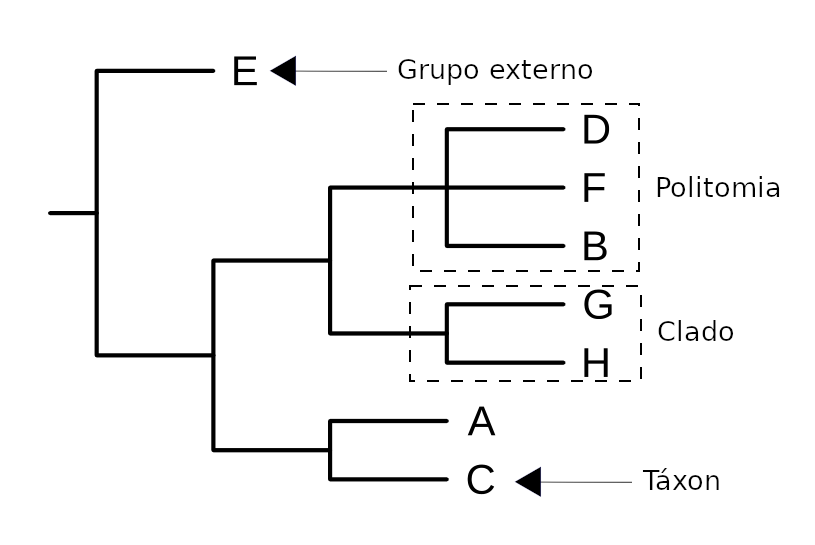
\includegraphics[width=.8\textwidth]{img/phylogeny}
  \caption{Exemplo de árvore filogenética}
  \label{fig:phylogeny}
\end{figure}

Em uma análise filogenética, os táxons são representados por sequências de caracteres, \emph{strings} dentro de um alfabeto geralmente discreto em que cada símbolo representa uma característica do táxon que pode ser passada hereditariamente. Essas sequências podem ser formadas por trechos de DNA, aminoácidos de proteínas ou mesmo características fenotípicas, como aspectos morfológicos. Para que a análise funcione, as sequências de todos os táxons devem ter o mesmo tamanho, e cada posição deve representar a mesma característica. O conjunto de todas as sequências analisadas forma a matriz de caracteres \cite{bootstrap}.

O modelo assume que os táxons se diversificam ao longo do tempo em dois (ou mais) táxons descendentes pelo processo de evolução. Na árvore, essa relação fica representada pelos descendentes apresentados como nós filhos do táxon ancestral. Assume-se que o mais provável é que um táxon evolua apenas para dois descendentes, embora possam ser aceitos mais numa relação conhecida como \textbf{politomia}.

Uma filogenia pode ser enraizada ou não-enraizada. Em uma árvore filogenética enraizada, o tempo "flui" da raiz para as folhas, ou seja, quanto mais próximos das folhas, mais recentes são os táxons. Em uma árvore não-enraizada, não é possível determinar quais nós internos representam os táxons mais antigos. Uma árvore não-enraizada pode ter uma raiz atribuída com a inclusão de um \textbf{grupo externo} à análise, isto é, um conjunto de táxons que sabe-se ter divergido antes do grupo analisado, chamado de \textbf{grupo interno} \cite{felsenstein2004inferring}.

O objetivo de uma análise filogenética é encontrar a melhor filogenia para um determinado grupo de táxons, isto é, dada uma matriz $n \times m$ com $n$ táxons e $m$ caracteres, a análise retorna uma árvore com exatamente $n$ folhas que melhor representa a história evolutiva do grupo a partir de um determinado critério.

\subsection{Etapas de uma análise filogenética}

Os métodos para análises filogenéticas podem ser divididos em dois grupos principais: os baseados em distância e os baseados em sequências \cite{cotta2002inferring}. Métodos por distância agreagam iterativamente os clados mais próximos entre si baseados em alguma métrica absoluta, criando uma matriz de distâncias entre todos e resumindo cada táxon a um vetor de números. Fazem parte desse grupo os métodos UPGMA e Neighbor-Joining, por exemplo. Métodos baseados em sequências dependem da análise individual de cada caracter das sequências associadas aos táxons, com referência a algum critério. Análises por sequência podem ser divididas grosseiramente em quatro etapas: busca, avaliação, consenso e suporte. Essas etapas não necessariamente representam um processo linear e não são totalmente dissociadas, porém tal separação facilita a compreensão do método.

A etapa de busca consiste em determinar um método para percorrer o \emph{espaço de busca} de árvores filogenéticas, isto é, o espaço que contém todas as possíveis filogenias válidas para um determinado conjunto de táxons de entrada. Assume-se para esta etapa que apenas árvores binárias completas (sem politomias) são válidas. \cite{cavalli1967phylogenetic} calcularam o  tamanho do espaço das árvores não-enraizadas $U_n$ para um conjunto de $n$ táxons como
\begin{equation}
  U_n = (2n-5)!!,
\end{equation}
onde $!!$ representa a operação fatorial duplo. Para as árvores enraizadas o tamanho do espaço corresponde a 
\begin{equation}
  R_n = U_{n+1} = (2n-3)!!.
\end{equation}
Como o espaço para árvores não-enraizadas é menor, a maioria dos métodos foca nesse tipo, enraizando as respostas com a inclusão de grupos externos, se necessário.

Determinar a filogenia ótima, procurando por todos os elementos do espaço de busca, consiste em um problema NP-Difícil \cite{np-hardness}, tornando uma busca ingênua impraticável para mais do que alguns poucos táxons. Mesmo sem percorrer todo o espaço, usando métodos como \emph{branch and bound} \cite{branch-and-bound}, realizar uma busca exata (garantindo o resultado ótimo) ainda é muito custoso. Por essa razão, a maioria das análises utiliza métodos heurísticos, que consistem em trocar de lugar iterativamente ramos na melhor árvore encontrada até o momento, na esperança de achar um resultado melhor (algoritmos de \emph{hill climbing}). Alguns operadores comuns para essa busca são o TBR (\emph{tree bissection-reconnection}), o SPR (\emph{subtree prune-regraft}) e o NNI (\emph{nearest-neighbor interchange}) \cite{garli}.

A fase de avaliação ocorre intercaladamente com a fase de busca e permite analisar a qualidade de cada árvore gerada. Para isso, um critério de avaliação precisa ser definido. Os mais comuns são \emph{máxima parcimônia} (MP) \cite{maximum-parsimony}, que determina que as árvores que necessitam do menor número de passos evolutivos são as mais prováveis, e \emph{máxima verossimilhança} (MV) \cite{cavalli1967phylogenetic, maximum-likelihood}, que se baseia em modelos estatísticos de substituição dos caracteres para determinar a filogenia mais provável. Ambos os modelos apresentam benefícios e fraquezas para determinadas situações, mas todos são modelos simplificados de processos evolutivos e, portanto, não são capazes de refletir com fidelidade a realidade \cite{cavalli1967phylogenetic}.

A criação de uma árvore de consenso se faz necessária uma vez que a busca pode retornar mais de uma filogenia com a mesma avaliação, ou valores muito próximos dentro de um intervalo determinado. Surge então o desafio de quais clados serão mantidos para a resposta final. O método mais comum é o \emph{consenso estrito}, que determina que apenas os clados presentes em todas as filogenias obtidas pela busca devem ser mantidos na resposta final \cite{felsenstein2004inferring}. Note que ``colapsar'' clados exige quebrar a propriedade binária das árvores obtidas nas fases anteriores, gerando politomias. Outros métodos para consenso incluem a regra da maioria \cite{majority-rule} e o consenso de Adams \cite{adams}.

Por fim, é preciso avaliar a qualidade da solução obtida. Para essa finalidade, o método mais comum é o \emph{bootstrapping}, adaptado do campo da estatística por \cite{bootstrap}. Esse se baseia em replicar a análise diversas vezes, reamostrando os caracteres, utilizando sorteios com repetição, e medindo a porcentagem de análises nas quais os clados são obtidos. Clados com boas porcentagens representam chances altas de serem representativos no mundo real. Como alternativa, \emph{jackkniffing} realiza réplicas da análise descartando um caracter por vez.

No caso de buscas utilizando o critério de máxima parcimônia, o suporte de Bremer \cite{bremer-support} pode ser utilizado como complemento ao \emph{bootstrap}. Esse analisa quantas \textbf{homoplasias} são necessárias para que um clado seja eliminado do consenso, isto é, quantos passos evolutivos extras precisam ser considerados para que a filogenia seja desmanchada. Valores maiores representam maior robustez da resposta.

\subsection{Algoritmos genéticos}

Algortimos genéticos (AGs) pertencem a uma classe de algoritmos denominados \emph{evolutivos}, que se baseiam em princípios de evolução darwiniana para obter respostas para problemas computacionais. AGs funcionam codificando possíveis soluções para um problema de otimização em \emph{cromossomos} ou indivíduos, cujo conjunto forma uma população. Esses cromossomos são inicializados aleatoriamente e então recombinados entre si a cada iteração do algoritmo, gerando novas respostas. Cada novo cromossomo também está sujeito a mutações, pequenas alterações estocásticas que podem ocorrer em cada pedaço da resposta. Dois cromossomos são escolhidos para recombinação baseados em um critério de \emph{aptidão}, que determina a qualidade da solução. Cromossomos mais aptos devem escolhidos mais vezes, mas dependem da escolha eventual de respostas não-ótimas para manter uma certa ``variabilidade genética'' na população \cite{garli}. Os operadores de seleção, recombinação e mutação precisam ser definidos para cada problema.

Em comparação a métodos de \emph{hill climbing}, algoritmos genéticos são menos propensos a ficar presos em ótimos locais \cite{garli}. Isso é proporcionado tanto pela inclusão de cromossomos sub-ótimos na recombinação, quanto pela inclusão de pequenas variações individuais por meio das mutações. AGs também são particularmente úteis em problemas multiobjetivo \cite{mo-phylogenetics}. No entanto, por dependerem de fatores aleatórios, não são facilmente reprodutíveis e podem necessitar de várias execuções independentes para obter respostas consistentes. Também dependem de vários hiperparâmetros (tamanho das populações, taxas de mutação e recombinação, número de gerações etc.), e não garantem a resposta ótima, podendo igualmente cair em ótimos locais, bem como não atingir convergência.

No contexto de filogenia, algoritmos genéticos podem ser usados para a etapa de busca de métodos baseados em sequência, servindo como alternativa às buscas utilizando \emph{hill climbing}. Como cromossomos, podem ser utilizadas as várias topologias possíveis de árvores, ou mesmo codificações em vetores lineares das mesmas \cite{cotta2002inferring}. Já os clássicos SPR, TBR e NNI podem ser adaptados como operadores de mutação, enquanto o operador PDR (\emph{prune-delete-regraft}) pode ser utilizado para recombinação.

\section{Trabalhos relacionados}

\cite{parsigal} apresenta o \emph{software} PARSIGAL, que realiza buscas utilizando algoritmos genéticos para encontrar topologias candidatas e heurísticas de \emph{hill climbing} para alterar os candidatos, avaliando a melhor filogenia pelo critério de máxima parcimônia. O trabalho também apresenta diversas otimizações feitas na linguagem C para o cálculo da parcimônia de uma árvore. Também é apresentado o algoritmo PDR como operador de recombinação.
  
\cite{cotta2002inferring} comparam diversos métodos para obter filogenias baseadas em distâncias usando algoritmos evolutivos. Os autores compararam o uso da estrutura da árvore e codificações em \emph{strings} numéricas como cromossomos para o algoritmo, chegando à conclusão de que, para a maioria dos casos, a representação em árvore obtém maior acurácia.

Em \cite{mo-phylogenetics}, os autores utilizam o algoritmo de otimização multiobjetivo NSGA-II para implementar o \emph{software} MO-Phylogenetics, capaz de realizar análises filogenéticas baseadas em máxima parcimônia e máxima verossimilhança simultaneamente, retornando árvores ótimas via fronteira de Pareto. Já \cite{mo-phynet} estendem a aplicação do método para redes filogenéticas, modelos evolutivos que aceitam a transmissão de informações entre ramos que já divergiram, ampliando as possibilidades de usos da inferência multiobjetivo através do \emph{software} MO-PhyNet.

A partir da análise baseada em máxima verossimilhança, a tese de \cite{garli} explica em detalhes um algoritmo genético utilizando apenas mutações (sem recombinações), compilado no \emph{software} GARLI. Também são apresentados diversos \emph{benchmarks} do método em comparação a \emph{softwares} tradicionais, medindo, entre outros aspectos, a acurácia da busca e o tempo de execução. No mesmo trabalho, ainda é apresentada a variante p-GARLI, utilizando diversas populações com intercâmbio de indivíduos rodando em paralelo, a fim de permitir buscas simultâneas na mesma ordem de tempo da versão sequencial. \cite{parallel-gaml} também apresentam uma versão paralela do \emph{software} GAML, porém focando na paralelização do cálculo de aptidão de cada população. \cite{gatc} utilizam um algoritmo genético para prever e corrigir filogenias por MV em conjunto com o modelo ``Duplication-Transfer-Loss''.

Com outros algoritmos de busca, \cite{azouri2021harnessing} desenvolveram um método para inferência filogenética otimizando a escolha de passos em uma busca heurística usando \emph{random forest}. Já \cite{berger2010accuracy} demonstram um método de inclusão de táxons fósseis, codificados por morfologia, em uma árvore obtida previamente por máxima verossimilhança com sequências moleculares de táxons viventes.

% \textcolor{red}{Talvez citar também \cite{gatc}}

\section{\emph{Softwares} atuais}

Entre os \emph{softwares} de análise filogenética, a maior parte dos artigos consultados usa PAUP* \cite{paup}, podendo realizar buscas pelos critérios de máxima parcimônia, verossimilhança ou por métodos baseados em distância. Já o TNT \cite{tnt} é focado em análises por parcimônia e contém uma implementação do algoritmo de avaliação de Máxima Parcimônia de Pesos Implícitos \cite{iwmp}, ou MPPI, que atribui pesos aos caracteres da análise proporcionalmente à quantidade de homoplasias que esses apresentam em uma determinada árvore.

Para análises sob o critério de máxima verossimilhança, além do PAUP*, o programa RAxML \cite{raxml} tem ampla aplicação, devido ao uso de algoritmos de rápida execução, em conjuntos grandes de dados. O \emph{software} PhyML \cite{phyml} também é bastante utilizado, originalmente aplicando o operador NNI para as buscas heurísticas. O mesmo também faz uso de cálculos de parcimônia para eliminar árvores pouco promissoras.

Além dos métodos mais tradicionais já elaborados, uma técnica que vem ganhando espaço é o uso de Inferência Bayesiana (IB)\cite{tschopp2018challenges}, partindo de técnicas de MCMC, como Metropolis-Hastings. Alguns dos \emph{softwares}  que permitem o uso de caracteres morfológicos por essa técnica são o MrBayes \cite{mr-bayes} e o BEAST \cite{beast}. Embora relativamente recentes, \cite{mongiardino2021fossils} demonstraram que o modelo ``Fossil Birth-Death rate'', cominado com IB, pode produzir bons resultados para matrizes com dados paleontológicos, enquanto \cite{implied-ranting} comprovaram que o mesmo apresenta acurácia bastante próxima de análises por parcimônia em \emph{datasets} sintéticos. Já \cite{cau2017specimen} realizou com sucesso uma análise utilizando BEAST 2 \cite{beast-2} para filogenia de peixes Dipnoi a nível de espécime.

\section{Experimentos preliminares}

Para fins de demonstração dos métodos atuais usados em análises filogenéticas, os dados de três trabalhos de filogenia foram testados. As matrizes de cada publicação apresentam características distintas, como tipo e quantidade de caracteres, bem como quantidade de táxons e de dados faltantes, de forma a demonstrar os desafios de se realizar inferência filogenética, revelando como os dados demandam processos diferentes.

A análise de \cite{dicynodonts-cris} apresenta uma matriz de caracteres morfológicos cranianos e pós-cranianos de dicinodontes, um grupo extinto de répteis parentes dos mamíferos atuais. O objetivo era encontrar o posicionamento da espécie brasileira \emph{Jachaleria candelariensis} na árvore deste grupo. A busca original foi feita por \emph{branch and bound}, pelo critério de máxima parcimônia. A matriz de caracteres consiste em 14 táxons, sendo dois pertencentes ao grupo externo, com 44 caracteres. Como resultado original, foi obtido um consenso estrito a partir de seis árvores igualmente parcimoniosas, com 111 passos cada. 

O artigo de \cite{bremer-support} apresenta a ideia por trás do suporte de Bremer. Neste trabalho, o autor exemplifica a ideia de um estudo de caso com dois alinhamentos de sequências de RNA de plantas angiospermas: um com nove sequências de 64 nucleotídeos e outro com seis sequências de 82 nucleotídeos. Em ambos os casos, um táxon (Poacea) foi reservado como grupo externo. As buscas foram feitas por método exato e pelo critério MP. A análise da primeira matriz retornou duas árvores de 151 passos, enquanto a segunda retornou uma filogenia de 161 passos.

Por fim, o trabalho de \cite{cryolophosaurus} faz uma descrição osteológica completa dos fósseis do dinossauro \emph{Cryolophosaurus ellioti}. A partir dos dados obtidos por esse processo, uma análise foi realizada para determinar sua posição filogenética dentro do grupo Theropoda. A matriz usada apresenta 347 caracteres, com 56 táxons amostrados (seis no grupo externo). Essa enorme quantidade de dados só pode ser processada por métodos heurísticos, de forma que os autores optaram por realizar a busca usando o algoritmo TBR no programa PAUP* com 25000 réplicas de sequência de adição aleatória. O consenso resultante da avaliação por MP consiste em 108 árvores de 833 passos, agrupadas por consenso estrito e de Adams, com o mesmo resultado. Suportes por \emph{bootstrapping} e Bremer também foram calculados.

Para os testes, foi utilizado o \emph{software} TNT na versão 1.6. As análises de terópodes foram feitas utilizando a opção ``Traditional search'', que corresponde à análise por \emph{hill climbing}, com os resultados das matrizes menores (dicinodontes e angiospermas) sendo calculados com a opção ``Implicit enumeration'' (\emph{branch and bound}, busca exata). Em todos os casos, os caracteres foram configurados como discretos e não-ordenados. Foram testados tanto o critério de máxima parcimônia padrão quanto parcimônia de pesos implícitos (função de concavidade padrão, $k = 3$). Todas as árvores foram agregadas utilizando consenso estrito.
% e os suportes foram calculados por \emph{bootstrap} e Bremer.
Por simplicidade, não foram calculados valores de suporte nem índices de convergência e retenção.

\subsection{Resultados}

A filogenia obtida pelos dados de dicinodontes usando máxima parcimônia padrão (MPP) está presente na Figura \ref{fig:dicynodons-smp}. O resultado é exatamente o mesmo descrito no artigo original, à exceção de que a busca forçando a monofilia do grupo interno (obrigando-o a ser um clado exclusivo, sem nenhum táxon do grupo externo) retornou apenas quatro árvores, em vez das seis descritas. O algoritmo retorna seis árvores caso seja permitido que o gênero \emph{Lystrosaurus} esteja presente dentro do grupo interno, formando uma politomia na base do mesmo.

Já a busca utilizando pesos implícitos, presente na Figura \ref{fig:dicynodons-iwmp}, obteve um consenso um pouco mais resolvido de três árvores com pontuação 11,55, no qual os gêneros \emph{Wadiasaurs} e \emph{Kannemeyeria} deixaram de fazer parte da politomia na base do grupo interno e passam a enraizar um novo clado seguido pelo mesmo clado enraizado por \emph{Dinodontosaurus} na análise anterior. Por não haver cálculo de suportes para esse exemplo, e por falta de uma explicação com fundamentação biológica, fica difícil precisar a coerência desse resultado.

\begin{figure}[ht]
  \centering
  \begin{subfigure}{.4\textwidth}
    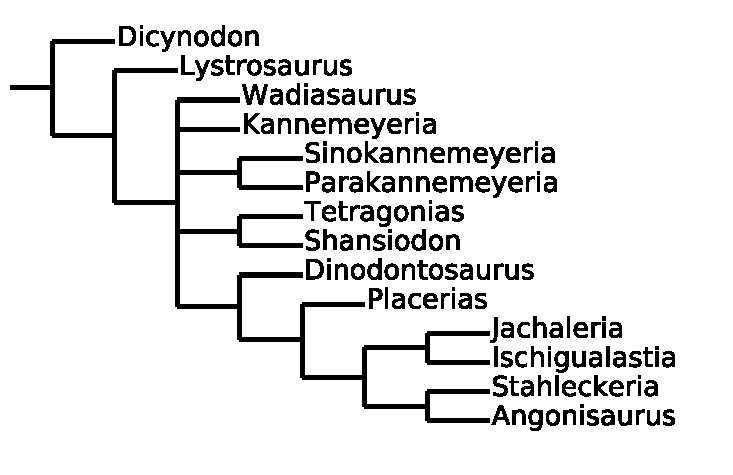
\includegraphics[width=\textwidth]{img/dicynodons-smp_svg-tex.pdf}
    \caption{Máxima parcimônia padrão}
    \label{fig:dicynodons-smp}
  \end{subfigure}
  \begin{subfigure}{.4\textwidth}
    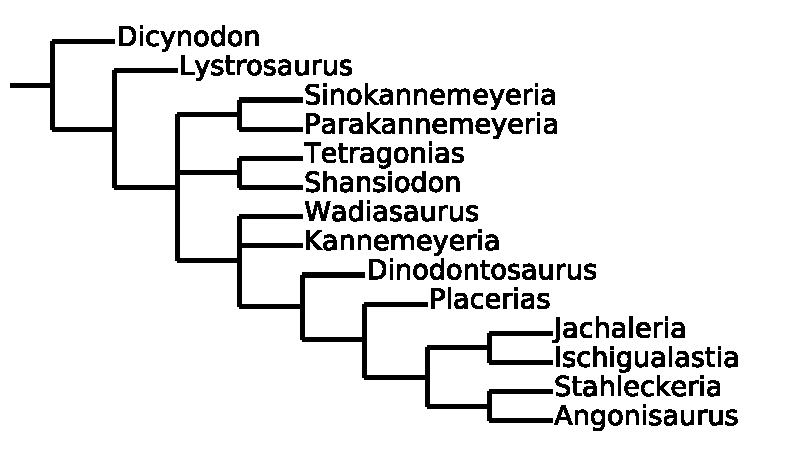
\includegraphics[width=\textwidth]{img/dicynodons-iwmp_svg-tex.pdf}
    \caption{Máxima parcimônia de pesos implícitos}
    \label{fig:dicynodons-iwmp}
  \end{subfigure}
  \caption{Árvore de consenso do \emph{dataset} de dicinodontes.}
  \label{fig:dicynodons}
\end{figure}

As árvores obtidas pelos alinhamentos de sequência de angiospermas avaliadas por MPP, tanto de nove (Figura \ref{fig:angiosperms-smp}) quanto seis táxons (Figura \ref{fig:angiosperms2}), resultaram exatamente nas filogenias descritas originalmente. Como ambos os trabalhos foram realizados por buscas exatas, é de se esperar que os valores de suporte também sejam os mesmos. Já a análise usando MPPI no alinhamento de nove táxons, apresentado na Figura \ref{fig:angiosperms-iwmp}, mostra algumas diferenças significativas em relação ao resultado original, com a família Asteracea na base do grupo interno e Apiacea como grupo irmão de Chenopodiacea. No entanto, como o suporte de Bremer do resultado original já era baixo ($\leq 3$), também pode se esperar que o suporte nesse caso seja baixo. A aplicação de MPPI no \emph{dataset} de seis táxons não obteve nenhuma diferença do original.

\begin{figure}[ht]
  \centering
  \begin{subfigure}{.4\textwidth}
    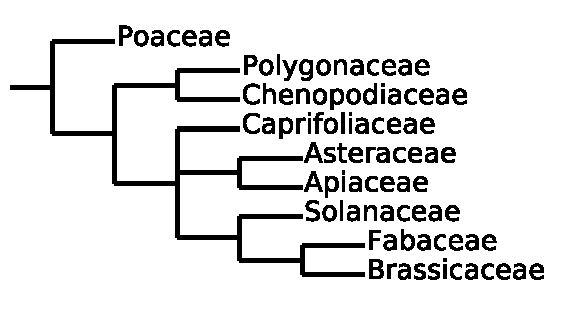
\includegraphics[width=\textwidth]{img/angiosperms-smp_svg-tex.pdf}
    \caption{9 táxons -- MPP}
    \label{fig:angiosperms-smp}
  \end{subfigure}
  \begin{subfigure}{.4\textwidth}
    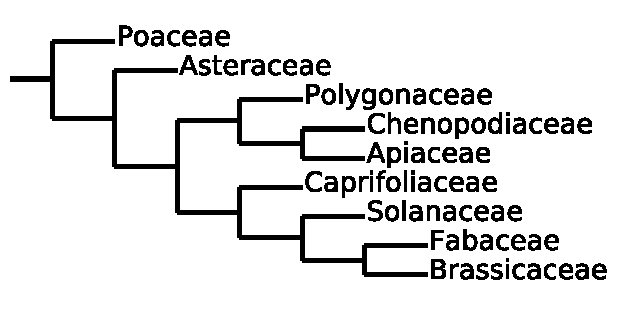
\includegraphics[width=\textwidth]{img/angiosperms-iwmp_svg-tex.pdf}
    \caption{9 táxons -- MPPI}
    \label{fig:angiosperms-iwmp}
  \end{subfigure}
  \begin{subfigure}{.4\textwidth}
    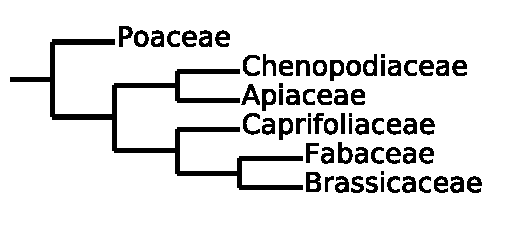
\includegraphics[width=\textwidth]{img/angiosperms2_svg-tex.pdf}
    \caption{6 táxons -- MPP e MPPI}
    \label{fig:angiosperms2}
  \end{subfigure}
  \caption{Árvore de consenso dos \emph{datasets} de angiospermas.}
  \label{fig:angiosperms}
\end{figure}

Por fim, a análise da matriz geral de terópodes sob o critério de máxima parcimônia padrão (Figura \ref{fig:theropods-smp}) obteve um resultado bastante similar ao reportado originalmente, embora os números obtidos tenham sido significativamente diferentes. Em vez das 108 árvores originais de 833 passos, foram retornadas apenas oito árvores de 853 passos. O número reduzido de árvores, similar ao ocorrido no caso dos dicinodontes, é provavelmente um artefato da monofilia forçada no relatório oferecido pelo TNT, enquanto o valor das árvores mais parcimoniosas possivelmente se deve a limitações de memória do \emph{software}. Em relação ao consenso obtido, a única diferença em relação ao original foi o posicionamento do gênero \emph{Coelurus}, que passou a integrar a posição mais ancestral em (\emph{Coelurus} + ``Paraves''). O resultado da análise com o critério MPPI (Figura \ref{fig:theropods-iwmp}) retornou três árvores com pontuação $\approx 80,76$, cuja maior diferença em relação à analise por MPP se dá nos posicionamentos dentro do clado Spinosauroidea. 

\begin{figure}[ht]
  \centering
  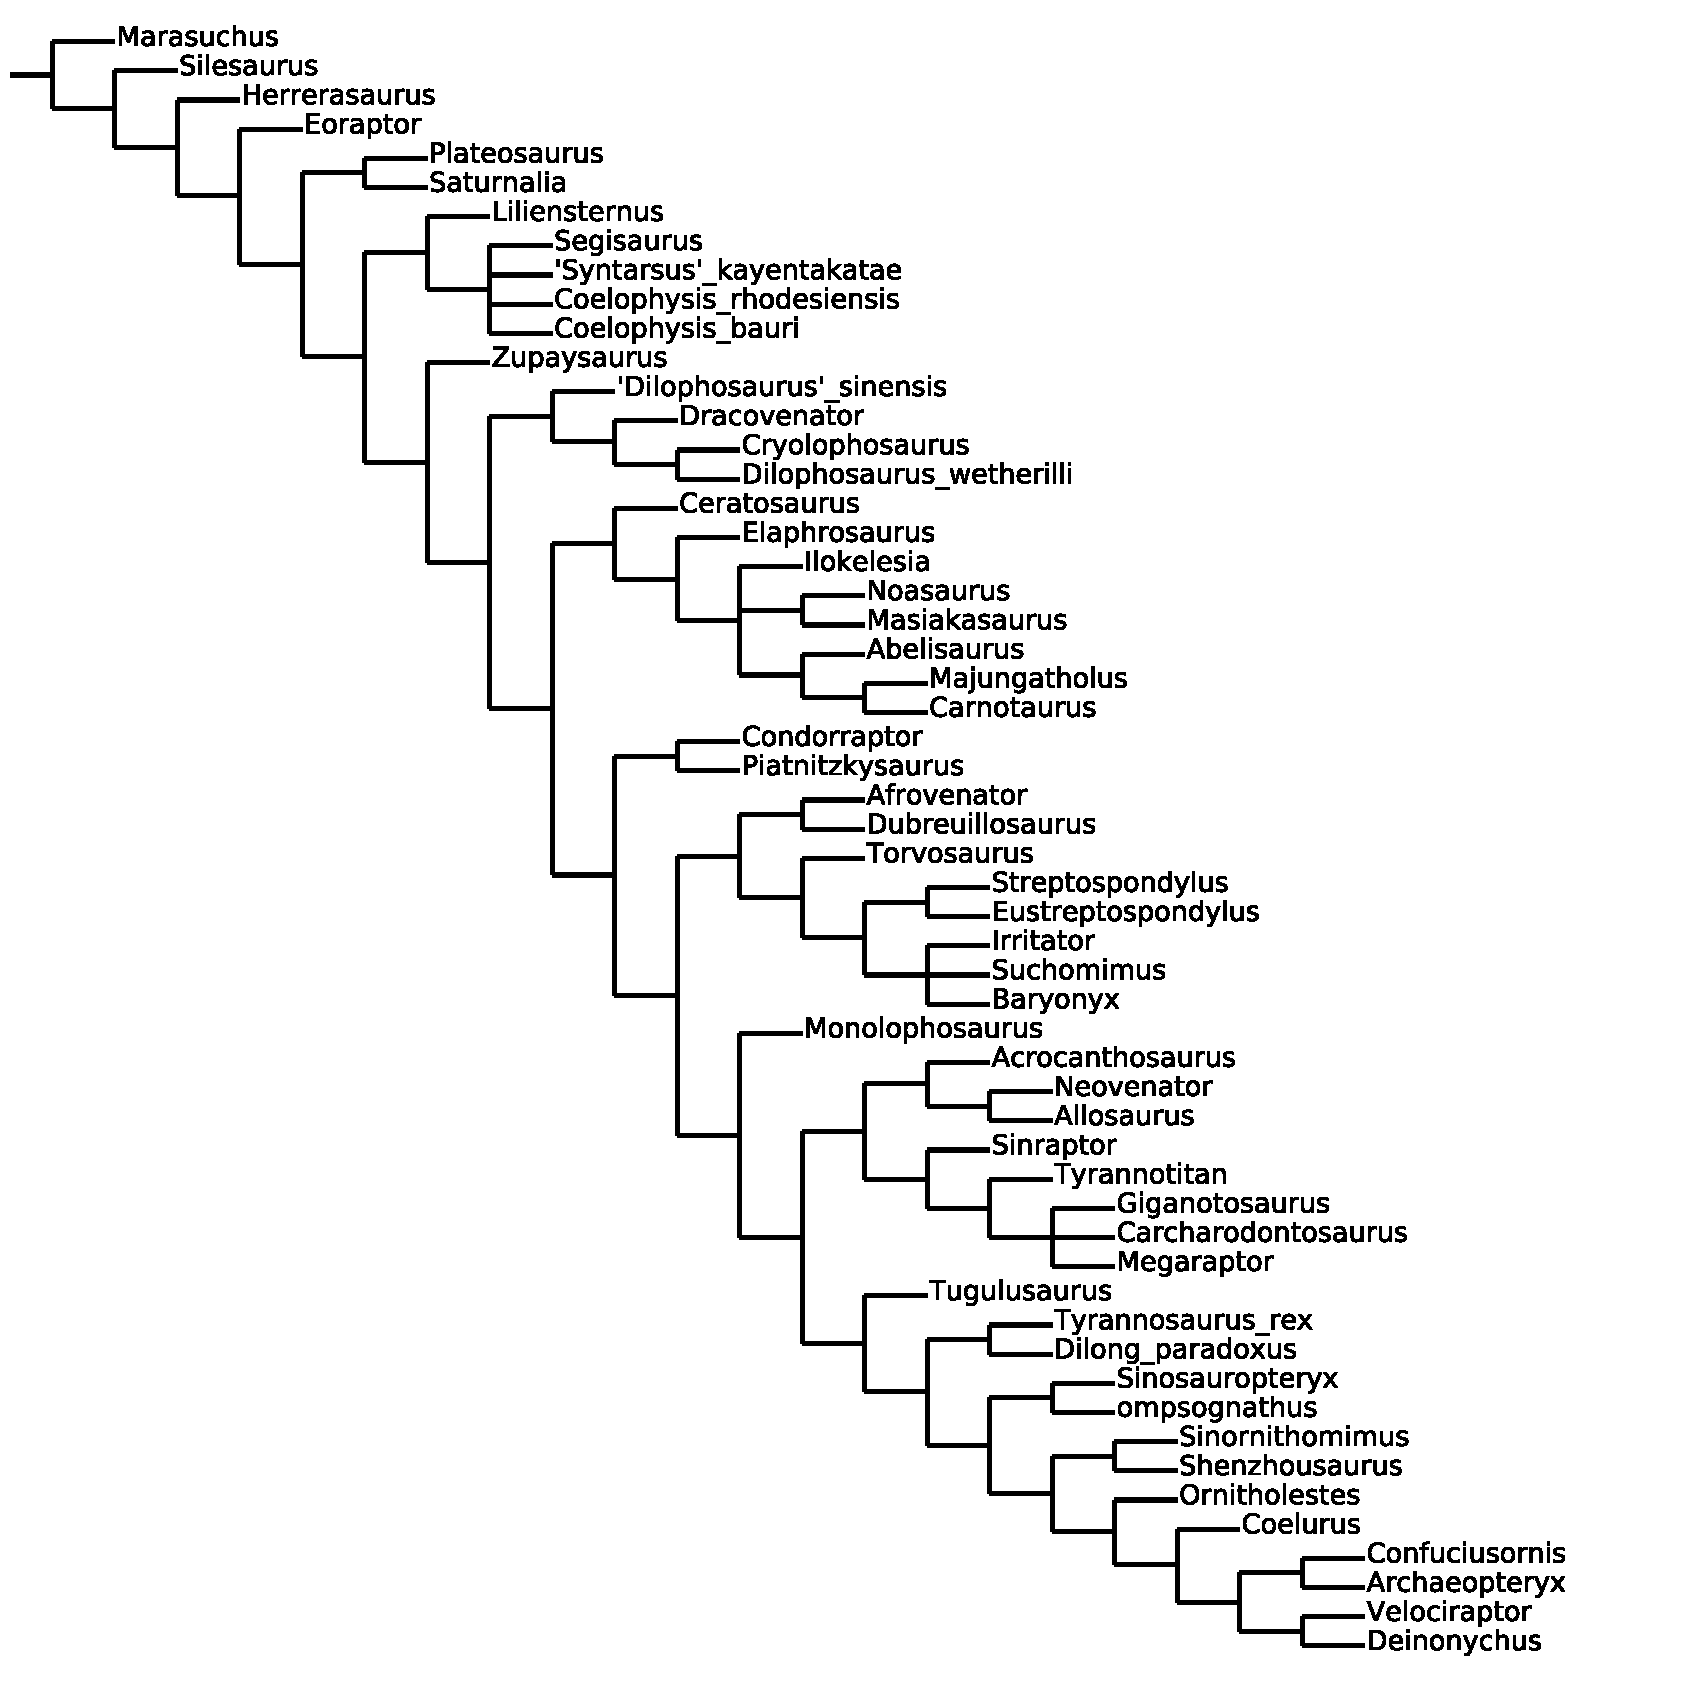
\includegraphics[width=\textwidth]{img/theropods-smp_svg-tex.pdf}
  \caption{Árvore de consenso do \emph{dataset} de terópodes sob o critério de máxima parcimônia padrão}
  \label{fig:theropods-smp}
\end{figure}
\begin{figure}[ht]
  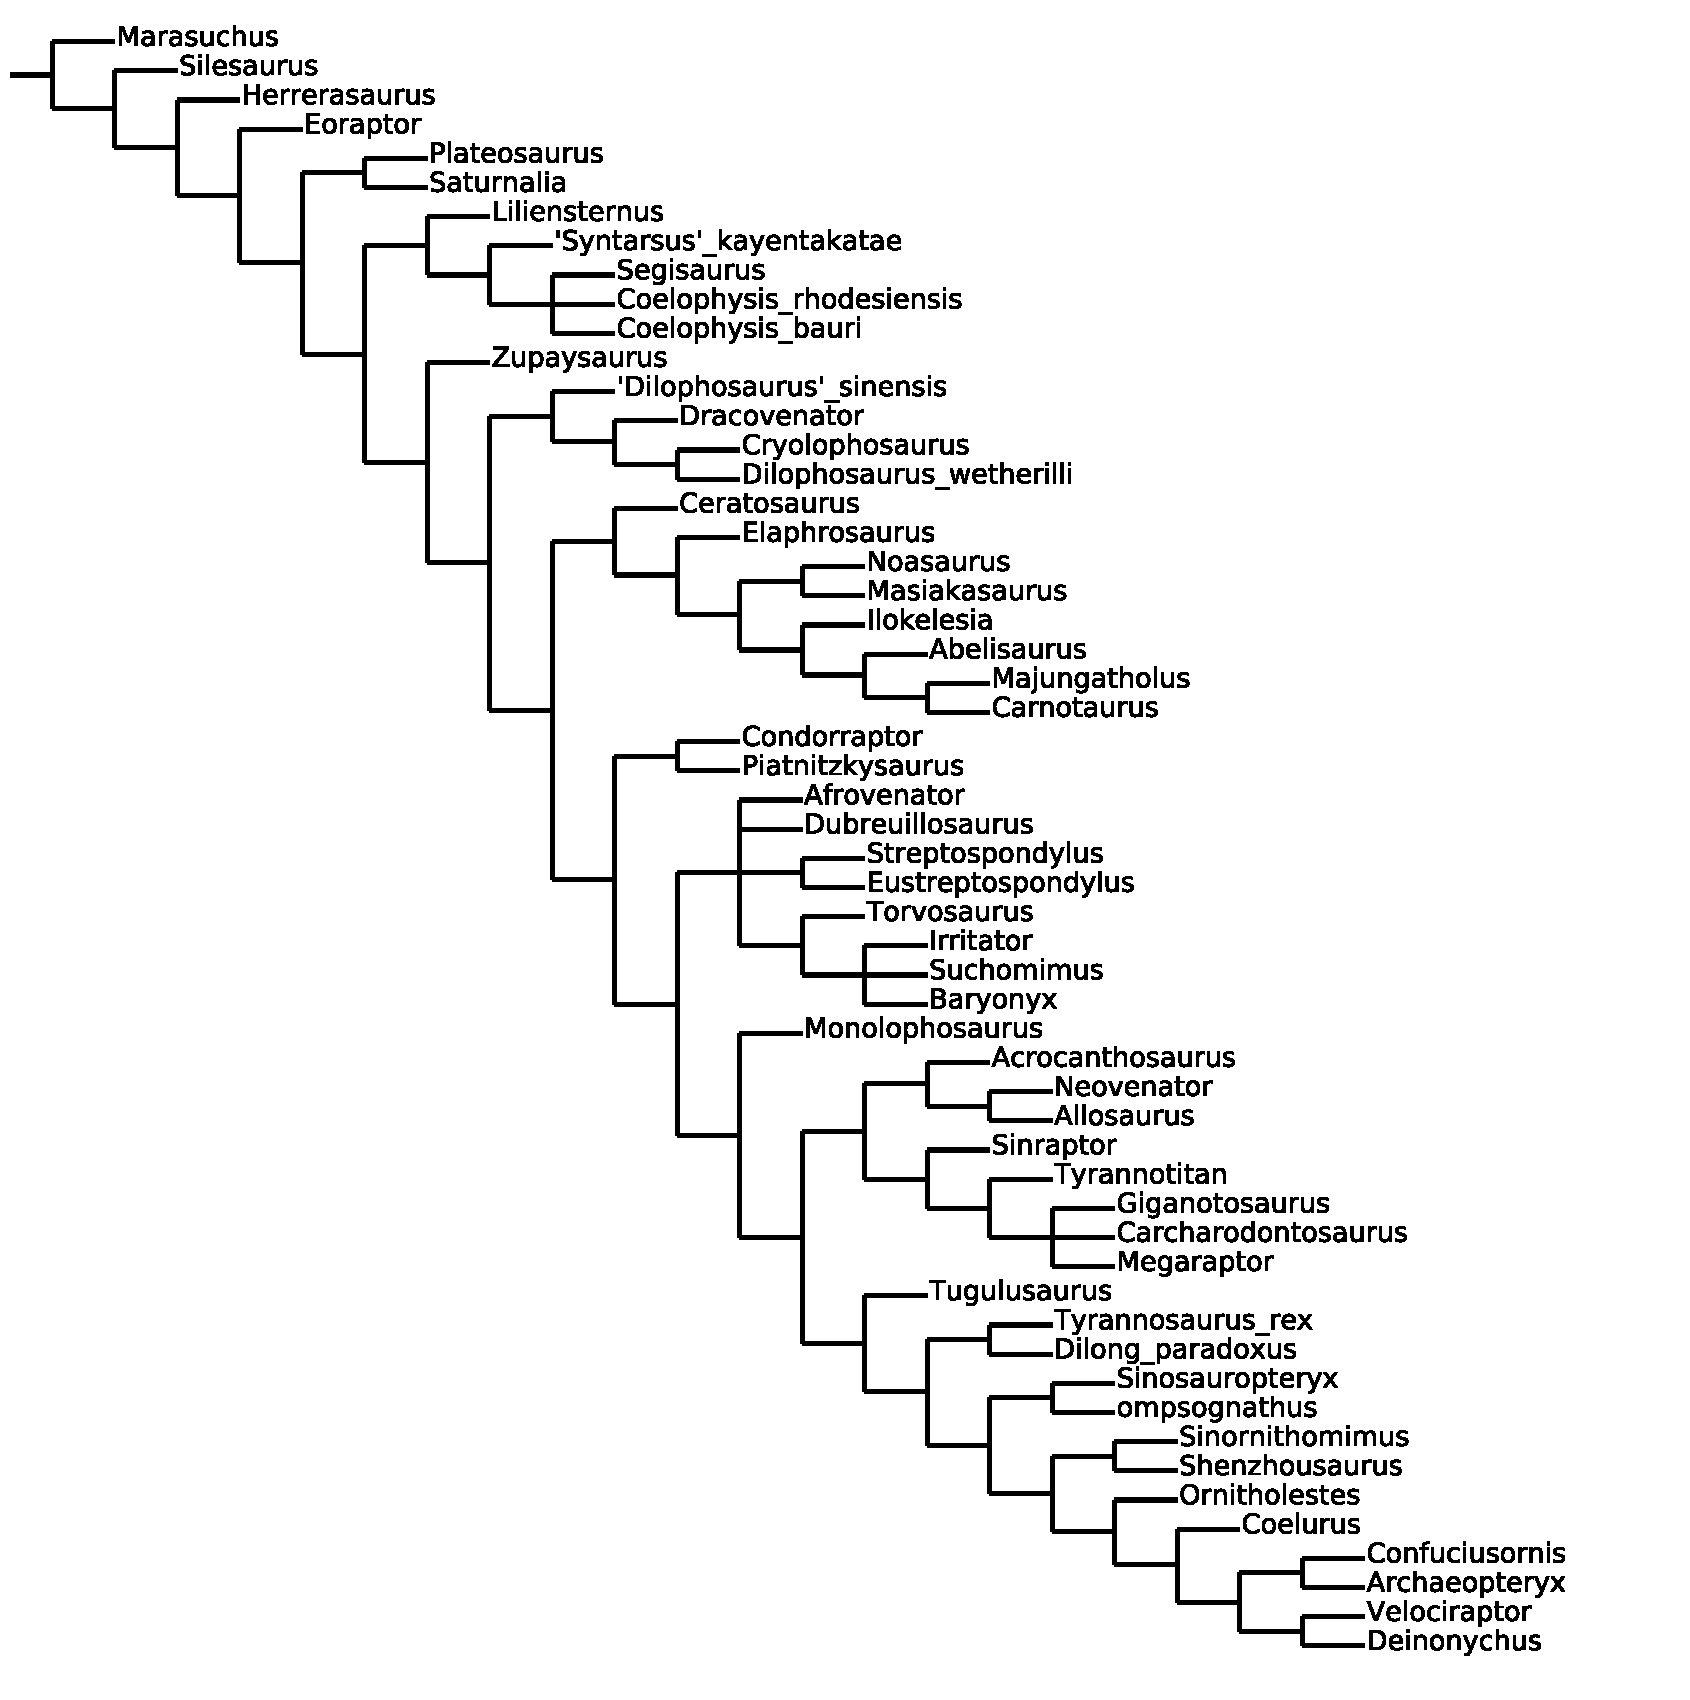
\includegraphics[width=\textwidth]{img/theropods-iwmp_svg-tex.pdf}
  \caption{Árvore de consenso do \emph{dataset} de terópodes sob o critério de máxima parcimônia de pesos implícitos}
  \label{fig:theropods-iwmp}
\end{figure}

\section{Proposta de trabalho}

Para este trabalho, a proposta consiste na elaboração de um algoritmo genético para busca de árvores filogenéticas, utilizando como entrada matrizes de caracteres morfológicos sob o critério de máxima parcimônia. O algoritmo será testado utilizando tanto bases de dados sintéticas, cuja resposta correta pode ser determinada, mas que apresentam baixa correspondência com problemas reais; quanto com bases de dados reais retiradas de artigos da área de Paleontologia, cuja acurácia apenas pode ser obtida em relação aos resultads publicados e aplicação de outros métodos semelhantes.

O algoritmo será baseado principalmente em três dos trabalhos citados: no \emph{software} GARLI de \cite{garli}, utilizando-se majoritariamente de operadores de mutação, hiperparâmetros definidos para o \emph{software} e método de avaliação dos resultados obtidos; e nos trabalhos de \cite{cotta2002inferring} e \cite{parsigal}, adaptando o operador de recombinação PDR e possivelmente, utilizando as codificações de cromossomos e otimizações de código desenvolvidas para ambos os trabalhos. Para as análises, serão utilizadas avaliações por MP tanto convencional quanto de pesos implícitos, aplicadas como funções de aptidão para o AG. O consenso será calculado de forma estrita, e os suportes deverão se basear em \emph{bootstrapping} e pelo método de Bremer. O algoritmo será comparado com buscas \emph{hill climbing} tradicionais sob o mesmo \emph{framework}, bem como com o algoritmo de \emph{branch and bound}, quando cabível.

Além da acurácia da resposta, também serão coletadas outras métricas de desempenho do algoritmo, como distância para a resposta correta, tempo de execução, e possivelmente uso de memória e CPU. O objetivo é avaliar o custo do algoritmo em relação aos métodos tradicionais caso tenha acurácia superior aos já usados, ou mesmo identificar se gasta mais recursos com desempenho similiar. Para isso, é importante que todos os algoritmos sejam executados em uma mesma base de código, para eliminar ao máximo artefatos de implementação nesses resultados. Em último caso, o resultado pode ser comparado a \emph{softwares} existentes, como TNT e PAUP*.

Por fim, vale ressaltar que o objetivo deste trabalho não será desenvolver um \emph{software} completo de análise filogenética, mas sim testar o desempenho de algoritmos genéticos como mecanismos de busca para filogenias baseadas em dados paleontológicos. O desenvolvimento de uma ferramenta pronta para uso requer a elaboração de vários detalhes que não serão levados em conta para este trabalho, como otimizações de código, criação de interface de usuário intuitiva, habilitação de configurações para o usuário, entre outras. O objetivo é demonstrar (ou não) que há benefício na implementação futura de \emph{softwares} com esse conceito, e pavimentar o caminho para as próximas pesquisas na área de algoritmos genéticos para análises filogenéticas.

\section*{Reconhecimentos}
Este trabalho foi feito usando a versão 1.6 do software TNT, disponibilizado gratuitamente para usuários finais pela Willi Hennig Society.

\bibliographystyle{sbc}
\bibliography{relatorio-tcc1}

\end{document}
